% !TEX TS-program = pdflatex
%
% File acl2017.tex
%
%% Based on the style files for ACL-2015, with some improvements
%%  taken from the NAACL-2016 style
%% Based on the style files for ACL-2014, which were, in turn,
%% based on ACL-2013, ACL-2012, ACL-2011, ACL-2010, ACL-IJCNLP-2009,
%% EACL-2009, IJCNLP-2008...
%% Based on the style files for EACL 2006 by 
%%e.agirre@ehu.es or Sergi.Balari@uab.es
%% and that of ACL 08 by Joakim Nivre and Noah Smith

\documentclass[11pt,a4paper]{article}
\usepackage[hyperref]{acl2017}
\usepackage{times}
\usepackage{latexsym}
\usepackage{graphicx}
\graphicspath{ {pictures/} }
\usepackage{url}
\usepackage{amsmath}


\aclfinalcopy % Uncomment this line for the final submission
%\def\aclpaperid{***} %  Enter the acl Paper ID here

%\setlength\titlebox{5cm}
% You can expand the titlebox if you need extra space
% to show all the authors. Please do not make the titlebox
% smaller than 5cm (the original size); we will check this
% in the camera-ready version and ask you to change it back.

\newcommand\BibTeX{B{\sc ib}\TeX}

\title{Graphical model for Topic model}

\author{Rong Ye \\
	Affiliation / Address line 1 \\
	Affiliation / Address line 2 \\
	{\tt email@domain} \\\And
	Haonan Li \\
	Affiliation / Address line 1 \\
	Affiliation / Address line 2 \\
	{\tt email@domain} \\\And
	Keyong Huang \\
	Affiliation / Address line 1 \\
	Affiliation / Address line 2 \\
	{\tt email@domain} \\}

\date{6.29.2017}
\begin{document}

\maketitle
\begin{abstract}
Latent Dirichlet Allocation(LDA) is a popular algorithm for Topic Modelling, which is widely used in many fields like e-commerce, document summarised, etc. In this project, we're trying to realise the LDA via Gibbs Sampling in python and then conduct empirical analysis on three different tasks - document modelling, document classification and collaborative filtering(CF). And our results show LDA performs well in document modelling and CF, but unsatisfactory in document classification.
\end{abstract}

\section{Introduction}

The goal of topic modeling is to discern latent topics of a collection of documents. To specify, the project requires us to find the topic structures of the corpus according to the content based on the statistical relationship between them, which is useful in numerous tasks. LDA is a generative model based on the simple 'bag-of-words' assumption. The variations of LDA also raise a lot of attention in recent years. However, we will limit our passage only to the traditional LDA method and its applicaitions.   

The paper is organised as follows. In Section 2 we will introduce the basic idea of Latent Dirichlet Allocation(LDA) via Gibbs Sampling and how we implement it in Python. In Section 3, we will focus on the task of topic modeling. We will introduce the document classification in Section 4. In Section 5, we will present you with empirical result in collaborative filtering. 

%\section{Data Preprocessing}
%As the convention of natural language preprocessing, we remove stopwords 
%like 'we','us' in all documents and stem them afterwards. In order to make 

\section{Introduction and Implementation of LDA}

Latent Dirichlet Allocation(LDA) is a hierarchical model for topic modelling. Unlike simple algorithms like PLSI, LDA assume that a single document may comprise of several different topics.The graphical representation is as Figure1.The detailed explanation of LDA model can be found in Blei(2003).

\begin{figure}[h]
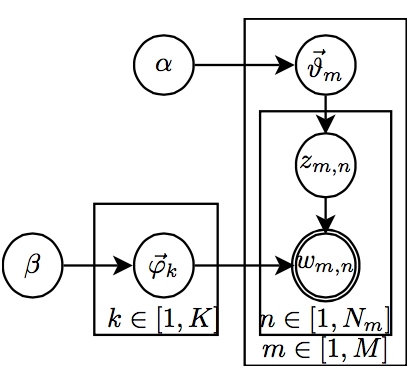
\includegraphics[scale=0.8]{graphic_rep.png}
\centering
\caption{Graphical Representation of LDA}
\centering
\end{figure}

The inference of posterior distribution can be considered in different ways. In this article, we will use Gibbs Sampling to implement LDA. The Gibbs Sampling is a popular Monte Carlo sampling method. The essence of this method is to compute the conditional distrition $P(z_i | x, z^{\neg}_i ) $, where $z^{\neg}_i$ indicates all z except $z_i$ for token i. After calculation, we have:

\begin{displaymath}
P(z_i | x, z^{\neg}_i ) \propto \frac{n^{t}_{k, \neg i} + \beta}{ \sum_{t=1}^{V} n^{t}_{k, \neg i}+ V\beta}
\frac{n^{k}_{m, \neg i} + \alpha}{ \sum_{k=1}^{V} n^{k}_{m}+ K\alpha}
\end{displaymath}

,where $n^{t}_{k, \neg i}$ means the number of tokens assigned to topic k excluding token i, $n^{k}_{m, \neg i}$  indicates the number of tokens assign to topic k in document m excluding token i, corresponding to topic-term matrix and document-topic matrix.

Meanwhile, the number of iteration of Gibbs Sampling should be carefully assigned to speed up the whole process. In hindsight, 500 is an optimal number for the stationary sampling.

Afterwards, we need computer two values of interest: the term distribution for each topic and the topic distribution for each document, namely $\theta_m$ and $\phi_k$, where m = $1,2, \dots, M$ and k = $1,2,\dots, K$. The result is as following:

\begin{displaymath}
\phi_{k,t}= \frac{n^{t}_{k} + \beta}{ \sum_{t=1}^{V} n^{t}_{k}+ V\beta}
\end{displaymath}
\begin{displaymath}
\theta_{m,k} =  \frac{n^{k}_{m} + \alpha}{ \sum_{k=1}^{K} n^{k}_{m}+ K\alpha}
\end{displaymath}

In terms of the parameter tuning, common criterion is the perplexity of the test datasets. However, due to the goal of the specific task, one may find some changes on the metric of perplexity more appropriate. Thus, we will introduce this metric in detail later when we introduce the tasks.

\section{Topic Modelling}

In order to figure out the most suitable number of topics according to the content and semanteme based on the statistical features, we need a large set of data to train the data. Furthermore, we ensured the accuracy of the algorithm by comparing with other graphic modeling algorithm.

\subsection{Data description}

The dataset we use is Amazon Fine Foods reviews, which consists of 568,454 reviews of fine foods from 256,059 users left up to Oct. 2012. Amazon fine food reviews dataset has the following attributes: \emph{ProductId, UserId�, ProfileName, HelpfulnessNumerator} (number of users who found the review helpful), \emph{HelpfulnessDenominator} (number of users who indicated whether they found the review helpful)�, \emph{Score} (rating of the product), \emph{Time}�, \emph{Summary} (brief summary of the review)� and \emph{Text} (text of the review).

In our document modeling and classification problem, we use text information, Summary and Text as the corpus to train and test the LDA model. Score, whose rating between one and five, is the categorical variable in the document classification model. By applying LDA model, we can use a dense document-topic matrix derived by LDA model to replace a sparse co-occurrence matrix, thus serving a function of dimensionality reduction.

However the original dataset is too large thus too time-consuming for us to train the LDA model, so we randomly choose 1500 reviews from 1478 users evaluating 1318 products.

\subsection{Choose appropriate number of topics}

Here we use perplexity to evaluate the language model. Perplexity is a measurement of how well a model for prediction, ie. the inability (uncertainty or confusion) in understanding the text.  In Blei(2003) , the perplexity is algebraically equivalent to the inverse of average log-probability for a test set of documents, and is computed as:
\begin{displaymath}
perplexity({{D}_{test}})=\exp \left\{ -\frac{\sum{\log P({{w}_{d}})}}{\sum{{{N}_{d}}}} \right\}\
\end{displaymath}

A lower perplexity means a lower uncertainty when predicting the unseen documents, indicating a better performance for prediction.

In this experiment, we separate the corpus into 90\% for training and 10\% for testing, and compute the perplexity under different number of topics. And then choose the topic number gives the lowest perplexity to do further analysis.
Choose topic number = 5, 10, 15, 20, 25, 30, 50, 75, 100.
Before defining the maximum number of iteration, we do convergence test for the Gibbs sampler.

\begin{figure}[h]
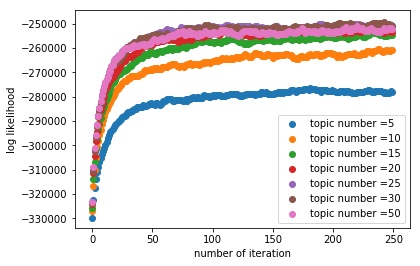
\includegraphics[scale=0.5]{converge_test.png}
\centering
\caption{Log-likelihood under 0-250 iterations}
\centering
\end{figure}

We plot the log likelihood under different number of iterations, from Figure 2, we can clearly find that after 250 iterations, the Gibbs sampler has already converge, and averagely speaking, for the document set of food review text, it will spend 2000 second(min = 1587s, max = 2796s) to train the LDA model and test it. Then we compute the perplexity for the 10\% test corpus under these topic numbers.

\begin{figure}[h]
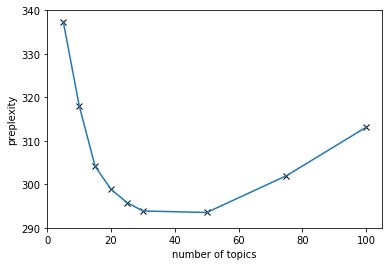
\includegraphics[scale=0.5]{num_perp_1.png}
\centering
\caption{Relationship between topic number and perplexity}
\centering
\end{figure}
Figure 3 shows that 50 topics give the lowest perplexity, but since the perplexity of 30 topics and 50 doesn?t vary much (perplexity(30) = 293.868, perplexity(50) = 293.521) and it spends less time when building a LDA topic model under 30 topics (Time(30) = 1990.05s ,time(50)  = 2212.37s), we choose 30 as the number of topics.


\subsection{Applications on comments text}

In each topic, we get the topic-vocabulary matrix represent the probability of the word given the topic. And we choose the ten largest probabilities of the words as the representative words of the given topic. The detailed result of 30 topics and their representative words is in the Appendix A.1. Here, in tabel 1, we showed some interesting topics and their representative words, and according to these representative words, we did manual annotation on the topics. Some of the topics are about the serves, like after-sale and delivery service in topic 1 and topic 18, some are about the category of products, like energy drink and coffee, and some are about the quality and health, etc.

\begin{table*}
\centering
\begin{tabular}{c|c|c}
\bf{Topic \#} & \bf{Representative words}& \bf{Manual Aspect} \\\hline\hline
\bf{Topic 1} & company, help, thought, please, stuff, change, huge, issue & After-sale\\\hline
\bf{Topic 3}  & drink, taste, ad, juicy, diet, want, energy, vitamin, like & Energy drink\\\hline
\bf{Topic 8}  &price, review, bag, great, brand, quality, new, know, deal & Price, quality\\\hline
\bf{Topic 11} & sweet, sugar, high, calories, fat, serve, low, protein, healthy & Sugar,fat\\\hline
\bf{Topic 18} & order, product, amazon, purchase, ship, item, receive, arrive, seller & Delivery\\\hline
\bf{Topic 27} & coffee, cup, pod, brew, roast, bold, strong, machine, Keurig & Coffee \\\hline 
\end{tabular}
\caption{Part of the topics, representative words and manual notation (based on LDA)}\label{tab:accents}
\end{table*}

\subsection{Test on other algorithms}
\label{ssec:other algo}
Since we have already had our own latent Dirichlet allocation algorithm, we want to test and compare the performance of other algorithm with ours. In order to do so, we need another graphic model to run the same data and differentiate their performance and find out the reason behind it, explain it.

The model we choose is probabilistic Latent Semantic Analysis model, in the short form: pLSA. The python library we used is Gensim. It is a robust open-source vector space modeling and topic modeling toolkit implemented in python. Once these statistical patterns are found, any plain text documents can be succinctly expressed in the new, semantic representation and queried for topical similarity against other documents.

\begin{figure}[h]
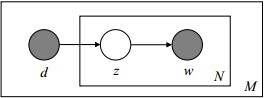
\includegraphics[scale=0.8]{plsa.png}
\centering
\caption{the graphical model of pLSA}
\centering
\end{figure}
,where d is document, z is the latent topic, w is word, N stands for the number of words, M for the number of documents. pLSI assumes that when generating a document, it follows the rules behind: First, randomly choose the picked specific topics from a set of topics. Secondly, randomly choose the words that belong to those topics. Continue these process until the number words picked meets the requirement.
\begin{displaymath}
\centering
P({{w}_{j}}|{{d}_{i}})=\sum\limits_{k=1}^{K}{P({{w}_{j}}|{{z}_{k}})P({{z}_{k}}|{{d}_{i}})}
\end{displaymath}
,where P(w|d) stands for the probability of the word chosen when the document has been decided, P(w|z) is the probability of a single word when the latent topic is chosen; P(z|d) is the probability of the occurrence of the topic given a document. Under this assumption, pLSA is the conversed process of the assumption. It uses the documents to inference the possible topics. That is the main idea of this algorithm. Table2 shows some of topics extracted from the outings. The detailed result of 30 topics and their representative words is in the Appendix A.2.

\begin{table*}
\centering
\begin{tabular}{c|c|c}
\bf{Topic \#} & \bf{Representative words}& \bf{Manual Aspect} \\\hline\hline
\bf{Topic 5} & hot, sauce, water, taste, type, use, like, again & Positive \\\hline
\bf{Topic 8}  & cookie, great, hot, chips, chocolate, price, eat, water & Energy food\\\hline
\bf{Topic 13}  & peanut, great, taste, butter, product, coconut, food & Breakfast\\\hline
\bf{Topic 26} & best, try, little, water, taste, smell, strong, enjoy & Like\\\hline
\bf{Topic 27} &Popcorn, chips, products, brand, free, gluten, amazon, little & snacks\\\hline
\end{tabular}
\caption{Part of the topics, representative words and manual notation based on pLSA}\label{tab:accents}
\end{table*}

Comparing to the previous our result of LDA model, it is obvious that pLSA model performs worse than our model. Actually, most of the topic words can not be assigned to a proper latent topic. 

\subsection{Possible explanations}
\label{ssec:explanations}

The most obvious difference between pLSA and LDA is that, at the document-topic level, all the variables are treated as parameters of the model, that is the number of the documents is the same as those parameters?. However, LDA introduces a hyper parameter, it models the document-topic level, using distributions to describe the probability. In training pLSA model, the value of parameters will increase together with the number of documents, and it can not generate model for new documents.

\section{Document Classification}

\subsection{Auto-tagging}
\label{ssec:tag}
According to the document-topic matrix and topic-vocabulary matrix, we can do auto-tag for a given text. From a Bayesian paradigm, we can compute the probability of each words given the certain document.
\begin{displaymath}
\centering
P(w|D)\text{=}\sum\limits_{z}{P(w|z)P(z|D)}
\end{displaymath}
,where w is the word, D is the given document and z is the topic. Choose the top 10 largest conditional probability as the tag of the given text D.

\subsection{Sentiment classification}
\label{ssec:clf}

We can infer the sentiment behind the food review, and these sentiments, whether satisfaction or discontent, can be somehow reflected on the score rating: from 1 to 5. Intuitively, when we score 1 or 2, we are unsatisfied, conversely, when rating 4 or 5, we are pleased with the service or product. Here, we divide the sentiment into \textbf{two categories}, and \textbf{three categories}.

\subsubsection{Application on Comment \emph{Text}}

We first classify the documents according to LDA model with feature, \emph{Text}.

{\bf Feature vector}: In original classification using word feature, we use 0-1 co-occurrence vector of a certain text as a feature vector, whose dimension is more than 2800. In a modified classification applying LDA model, we use the document-topic vector as a feature vector with a reduced dimension = 30 (as the analysis above, when topic number = 30, it gives the lowest model perplexity). 

Given that in the original word feature model, the length of feature vector is more than 2800, which is larger than sample size 1500, the classification model we use is \textbf{logistic regression} classifier.
~\\
{\noindent\bf Binary classification: positive and negative}

Denote negative attitude(score 1 or 2) as 0 and positive(score 3, 4 or 5) as 1.
\begin{displaymath}
\centering
\hat{P}=\frac{1}{1+{{e}^{-\hat{\mu }}}},\text{where }\hat{\mu }=\hat{\theta }x
\end{displaymath}
,where x is the feature vector. The decision boundary is {x: P = 0.5}.
Then we compute the accuracy of the classification under different proportion of the test set. Accuracy is defined as the proportion of the number of correct classification. 

The reduction in dimension certainly results in accelerating the LR classification. But when dealing with accuracy, as shown in Figure 5, LDA model fail to classification well.
\begin{figure}
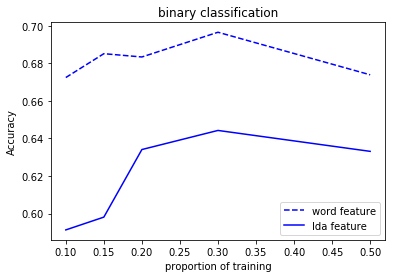
\includegraphics[scale=0.5]{2clf1.png}
\centering
\caption{Binary classification on comment text}
\centering
\end{figure}

~\\
{\noindent\bf Three-class classification: positive, neutral and negative}
Sometimes, score 3 is hard to define under 1-5 rating system, and in this case, we regard score 3 as a separate group ? neutral, thus making the classification a multiclass one. Traditionally, logistic regression is used in binary, and fortunately, we can still use one-vs-all logistic regression classifiers, training a single classifier per class, with the samples of that class as positive samples and all other samples as negatives (ie. decision tree + logistic regression).

\begin{figure}
	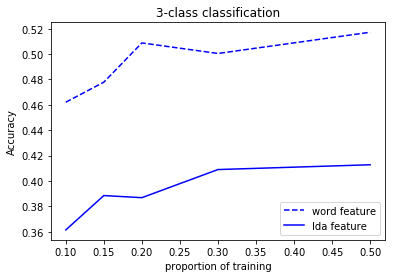
\includegraphics[scale=0.5]{3clf1.png}
	\centering
	\caption{Three-class classification on comment text}
	\centering
\end{figure}

From Figure6, disappointedly, the LDA model also doesn?t well in multi-classification problem.

We believe the major reason is that the word feature contains all the information of the document, but LDA feature, after all, is a compressed one. Besides, we guess another reason is partly due to the attribute we use ? Text, maybe text is a little bit long for LDA model to do classification, also running Gibbs LDA model on the review text too time-consuming. So, we decide to use shorter comment,\emph{Summary}, to do classification. 

\subsubsection{Application on Comment \emph{Summary}}

Just like the steps in the application on comment text, we first compute perplexity and choose the appropriate topic number, 10, the relation between LDA perplexity and topic numbers are shown in Figure 7, and 10 topics and their representative words are in Appendix A.3.

\begin{figure}[h]
	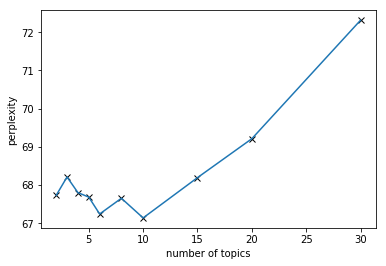
\includegraphics[scale=0.4]{choose_topic2.png}
	\centering
	\caption{Topic number and LDA perplexity on data \emph{Summary}}
	\centering
\end{figure}
Besides the original word feature, we also consider a new method dealing with the feature vector \text{-} Word2vec. \textbf{Word2vec} is also a method to reduce the dimension of the feature vector for classification, its main idea is to estimate the distance between the word and its context words in a document. To simplify, we just directly use word2vec in genism package. The classifier here is \textbf{Stochastic Gradient Descent (SGD)}, which is  commonly used  when the feature vector is sparse, and it is also a good classifier in NLP problems. 

~\\

{\noindent\bf Binary classification: positive and negative}
Same as what we did in Summary classification problem. Adding the Word2vec feature, we can get the result in Figure 8.
\begin{figure}
	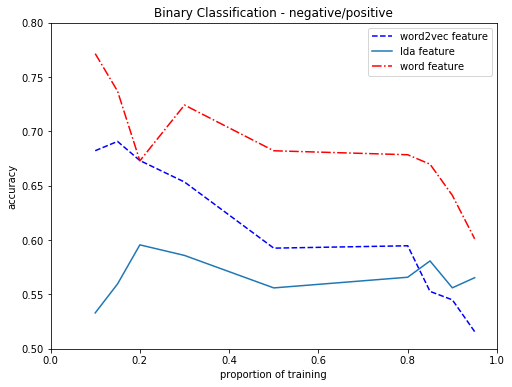
\includegraphics[scale=0.4]{2clf2.png}
	\centering
	\caption{Binary classification on comment \emph{Summary}}
	\centering
\end{figure}
From Figure 8, the original word feature is still the best one used in classification. However, the word feature is time consuming in the large-scale problems. Comparing word2vec feature and LDA feature, word2vec feature does pretty well when there isn?t much training data, and LDA feature is good after a large amount of trainings.

~\\
{\noindent\bf Three-class classification: positive, neutral and negative}

From figure 9, we find that the original word feature works much better than LDA and word2vec feature, and gives a super good performance in 3-class classification. Unlike the binary classification, LDA model works better than the word2vec feature with the low proportion of the training data. Nevertheless, whether LDA or word2vec, both are mediocre when dealing with multi-classification. 

\begin{figure}
	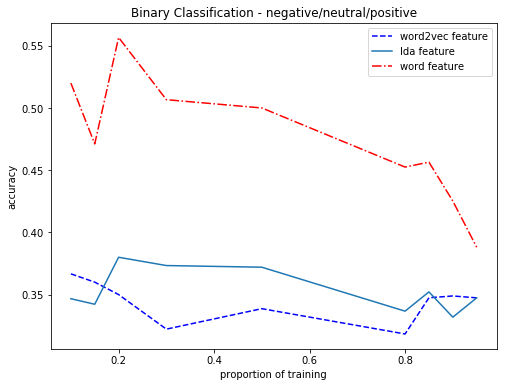
\includegraphics[scale=0.4]{3clf2.png}
	\centering
	\caption{Three-class classification on comment \emph{Summary}}
	\centering
\end{figure}

\subsection{The possible reasons that LDA model does not work well}
\label{ssec:resaon}

From the results and analysis above, no matter the long reviews or the short summaries, disappointedly, unlike the performance in Blei(2003), the LDA classification is not as good as original word feature, and this is partly because of the dataset we use. We simply choose 1500 comments from the whole dataset, which makes the data somewhat ?impropriate? for building model. For example, most of the 1318 products have only one review, thus making the topics untypical. Another problem is that the distribution of Score is not the same as the original dataset, which would also influence the performance of the LDA model. 

% Min: no longer used as of ACL 2017, following ACL exec's decision to
% remove this extra workflow that was not executed much.
% BEGIN: remove
%% \section{XML conversion and supported \LaTeX\ packages}

%% Following ACL 2014 we will also we will attempt to automatically convert 
%% your \LaTeX\ source files to publish papers in machine-readable 
%% XML with semantic markup in the ACL Anthology, in addition to the 
%% traditional PDF format.  This will allow us to create, over the next 
%% few years, a growing corpus of scientific text for our own future research, 
%% and picks up on recent initiatives on converting ACL papers from earlier 
%% years to XML. 

%% We encourage you to submit a ZIP file of your \LaTeX\ sources along
%% with the camera-ready version of your paper. We will then convert them
%% to XML automatically, using the LaTeXML tool
%% (\url{http://dlmf.nist.gov/LaTeXML}). LaTeXML has \emph{bindings} for
%% a number of \LaTeX\ packages, including the ACL 2017 stylefile. These
%% bindings allow LaTeXML to render the commands from these packages
%% correctly in XML. For best results, we encourage you to use the
%% packages that are officially supported by LaTeXML, listed at
%% \url{http://dlmf.nist.gov/LaTeXML/manual/included.bindings}
% END: remove


\section{Collaborative Filtering}

In our task of Collaborative Filtering(CF), we conduct LDA algorithm on the dataset from platform for movie reviewers ? MovieLens, to predict the preference of users and recommend them a new movie based on the their records. The dataset we are using is MoiveLens 20M(2016) and only a subset of it(2000 users in 138000) is included in our experiment due to the lack of computational resources. 

In our experiment, all users having less than 100 reviews are not included into our dataset in order to partly control the problem of sparsity. We divide this set of users into 1800 training users and 200 testing users. Training users will be further divided for the parameter tuning, which is number of topics in the LDA model. We train the model on a fully observed set of users. For each user in the test dataset, we hold out one movie in their records and use the others to guess the held-out movie. The evaluation metric is the likelihood of the held-out movie. More precisely, we define the predictive-perplexity as following:

\begin{small}
\begin{displaymath}
P\textrm{-}P(D_{test}) =  
 \exp{\left\{-\frac{\sum_{d=1}^M \log p(w_{d,N_d}|\mathbf{w}_{d,1:N_d-1})}{M}\right\}}
\end{displaymath}
\end{small}
\subsection{Model Training}

We split the training dataset into two groups, 80\% for modeling and 20\% for parameter tuning. And then we choose the best number of topics for our model via the predictive perplexity we achieve on the 20\% of training users. Result is as Figure:

\begin{figure}[h]
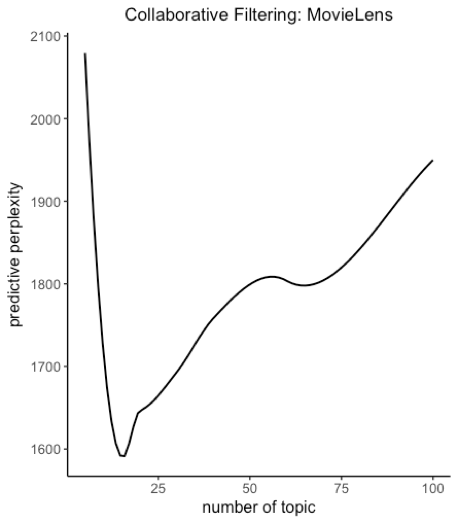
\includegraphics[scale=0.8]{cf_para_tune.png}
\centering
\end{figure}


we can see that the model with 15 topics predict the held-out movie best. Thus, we will use all data in training users to train the final model with 15 topics and check for performance on the testing users.

\subsection{Model Evaluation}
\label{sec:length}
Collaborative Filtering evaluation metric varies according to the goal of the tasks like whether you want to recommend the right items or annotate the message in the context. In our case, we will concentrate on finding the right items. One of effective metrics to evaluate recommendation system of this goal is to see the recall rate of this recommendation system versus the number of recommended movies. More precisely, we held out small part of the movies(1/5 in our case), and then we present user with M movies ranked by the probability they may exist in ones? profiles and evaluate based on which of these movies were actually in each users? profiles. The definition of recall rate can be defined as following:

\begin{displaymath}
recall\textrm{-}rate(M)=  \frac{M_{user\ likes} }{M_{held-out}}
\end{displaymath}

where $M_{user\ likes}$ is the the number of movies user likes and $M_{held-out}$ is the number of movies we held out for this user. The recommendation system recall rate will be the arithmetic average of recall rates or all users.

A Higher recall rate with lower M will be a better system. Besides, We also add a simple method using cosine to calculate the similarity between users to recommend them similar movies. We will take it as a baseline method to see how our LDA does in terms of the collaborative filtering. And the result is as Figure below.

\begin{figure}[h]
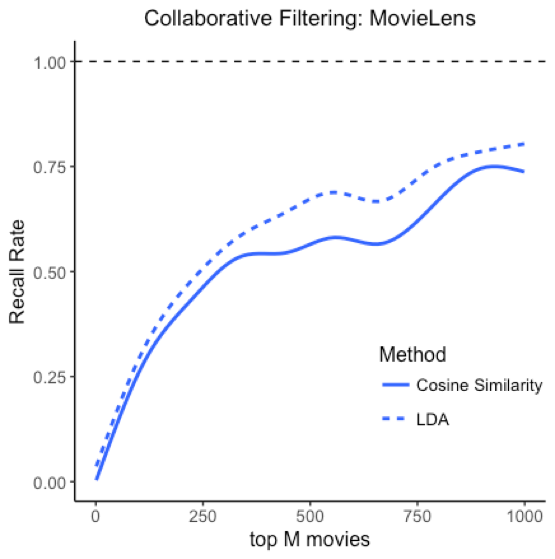
\includegraphics[scale=0.8]{cf_model_com.png}
\centering
\end{figure}

We can see that LDA does quite a good job and run much faster when the vocabulary is large compared with this traditional method, which needs to compute a large matrix. So LDA performs great in CF task when vocabulary is quite large compared with documents.

%\section*{Acknowledgments}

% include your own bib file like this:
%\bibliographystyle{acl}
%\bibliography{acl2017}
%\bibliography{acl2017}
%\bibliographystyle{acl_natbib}
\begin{thebibliography}{}
\bibitem[]{}McAuley, J. J., \& Leskovec, J. (2013, May). From amateurs to connoisseurs: modeling the evolution of user expertise through online reviews. In Proceedings of the 22nd international conference on World Wide Web (pp. 897-908). ACM.

\bibitem[]{}Heinrich G. Parameter estimation for text analysis (2005)[J]. Web: http://www. arbylon. net/publications/text-est. pdf, 2005.

\bibitem[]{}Blei D M, Ng A Y, Jordan M I. Latent dirichlet allocation[J]. Journal of machine Learning research, 2003, 3(Jan): 993-1022.

\end{thebibliography}

\appendix
\section{Appendix. Results of the programs(part)}
\label{sec:append}

In this appendix, we will show part of the results from the programs, including topic modeling using LDA and PLSA.

\subsection{30 Topics and their representative words in document classification}

As shown in table 3.

\begin{table*}[hp]
\centering
\begin{tabular}{c|c}
\textbf{Topic \#}  & \textbf{Representative words}                                              \\\hline\hline
\textbf{Topic 0:}  & tea , green , flavor , spice , bag , make , chai , leav , tast             \\
\textbf{Topic 1:}  & compani , help , thought , pleas , stuff , chang , huge , issu             \\
\textbf{Topic 2:}  & food , cat , eat , organ , year , babi , month , old , start               \\
\textbf{Topic 3:}  & drink , tast , ad , juic , diet , want , energi , vitamin , like           \\
\textbf{Topic 4:}  & dog , treat , love , recommend , chicken , anyth , feed , dri , quick      \\
\textbf{Topic 5:}  & tri , great , realli , bit , best , favorit , way , happi , nice           \\
\textbf{Topic 6:}  & product , ingredi , contain , list , syrup , natur , label , corn , addit  \\
\textbf{Topic 7:}  & good , better , star , pretti , bit , think , brand , someth , decent      \\
\textbf{Topic 8:}  & price , review , bag , great , brand , qualiti , new , know , deal         \\
\textbf{Topic 9:}  & box , packag , howev , open , pack , purchas , actual , sure , cost        \\
\textbf{Topic 10:} & enjoy , time , differ , fresh , worth , end , good , lot , notic           \\
\textbf{Topic 11:} & sweet , sugar , high , calori , fat , serv , low , protein , healthi       \\
\textbf{Topic 12:} & love , littl , peanut , butter , snack , think , good , eat , kind         \\
\textbf{Topic 13:} & bar , size , think , chew , eat , small , piec , half , larg               \\
\textbf{Topic 14:} & chocol , smell , like , someth , expect , nice , milk , bad , cream        \\
\textbf{Topic 15:} & hot , sauc , chees , spici , noodl , far , best , origin                   \\
\textbf{Topic 16:} & buy , bought , store , local , groceri , free , thought , gluten , cheaper \\
\textbf{Topic 17:} & flavor , tri , disappoint , fan , bad , good , realli , strong , hint      \\
\textbf{Topic 18:} & order , product , amazon , purchas , ship , item , receiv , arriv , seller \\
\textbf{Topic 19:} & like , look , got , thing , real , right , anoth , make , way              \\
\textbf{Topic 20:} & water , bottl , tast , want , recommend , acid , long , bodi               \\
\textbf{Topic 21:} & tast , like , better , quit , vanilla , milk , strong , sort , opinion     \\
\textbf{Topic 22:} & time , day , everi , need , realli , minut , noth , jar , wonder           \\
\textbf{Topic 23:} & cooki , amazon , product , com , ounc , pack , www , gp                    \\
\textbf{Topic 24:} & bag , oz , howev , know , come , pound , alway , read                      \\
\textbf{Topic 25:} & tast , like , chip , salt , popcorn , sure , definit , salti , pop         \\
\textbf{Topic 26:} & use , work , feel , wast , hair , brand , good , condition                 \\
\textbf{Topic 27:} & coffe , cup , pod , brew , roast , bold , strong , machin , keurig         \\
\textbf{Topic 28:} & appl , candi , tri , hope , help , want , ok , dri , stuff                 \\
\textbf{Topic 29:} & make , mix , littl , add , use , easi , coconut , rice , cook                                   
\end{tabular}
\caption{LDA topic modeling: 30 topics and their representative words}\label{tab:accents}
\end{table*}

\subsection{30 Topics and their representative words in document classification}

As shown in table 4.

\begin{table*}[hp]
\centering
\begin{tabular}{c|c}
\textbf{Topic \#} & \textbf{Representative words \& Probabilities}                                       \\\hline\hline
\textbf{Topic0:}  & coffee , like , tea , taste , would , one , its , good , product , love              \\
\textbf{Topic1:}  & coffee , dog , tea , food , coffee , cup , strong , coffee, , eat , treats           \\
\textbf{Topic2:}  & tea , coffee , tea , coffee , green , chai , dog , cup , tea, , teas                 \\
\textbf{Topic3:}  & dog , tea , coffee , food , treats , chocolate , taste , dogs , peanut , bars        \\
\textbf{Topic4:}  & price , dog , amazon , product , box , local , taste , grocery , eat , like          \\
\textbf{Topic5:}  & hot , sauce , water , taste , types , using , like , them , again , use              \\
\textbf{Topic6:}  & love , great , peanut , coffee , chips , water , free , \& , chocolate , like        \\
\textbf{Topic7:}  & chocolate , peanut , dog , love , butter , cats , food , best , sugar , chips        \\
\textbf{Topic8:}  & cookies , great , hot , chips , chocolate , cookie , price , them , eat , water      \\
\textbf{Topic9:}  & chips , chocolate , food , one , buy , great , bars , \& , dog , price               \\
\textbf{Topic10:} & \& , cookies , ive , chocolate , peanut , great , sauce , eat , water , cookie       \\
\textbf{Topic11:} & love , water , food , coffee , dogs , treats , easy , salt , hot , coconut           \\
\textbf{Topic12:} & product , peanut , chocolate , water , butter , price , food , dont , best , coconut \\
\textbf{Topic13:} & peanut , its , great , \& , taste , butter , would , product , coconut , food        \\
\textbf{Topic14:} & popcorn , coffee , drink , taste , like , easy , salt , coffee , really , \&         \\
\textbf{Topic15:} & chips , coconut , cup , sauce , great , coffee , coffee , product , eat , water      \\
\textbf{Topic16:} & flavor , best , water , ive , chips , one , box , its , would , taste                \\
\textbf{Topic17:} & mix , \& , product , peanut , gluten , price , good , best , water , dogs            \\
\textbf{Topic18:} & food , love , chips , best , cat , dog , cats , really , dogs , work                 \\
\textbf{Topic19:} & gluten , great , free , product , its , popcorn , \& , eat , healthy , easy          \\
\textbf{Topic20:} & buy , use , best , water , bought , local ,  , product , easy , cats                 \\
\textbf{Topic21:} & again , water , flavor , product , sauce , like , chocolate , drink , enjoy , \&     \\
\textbf{Topic22:} & \& , loves , chips , cup , buy , product , son , again , stars , baby                \\
\textbf{Topic23:} & coffee , popcorn , again , coffee , bold , tastes , \& , coconut , cup , love        \\
\textbf{Topic24:} & them , chips , price , really , its , eat , baby , bad , thought , flavor            \\
\textbf{Topic25:} & chai , make , bars , sure , would , cookies , every , think , \& , coffee            \\
\textbf{Topic26:} & best , tried , them , little , water , dogs , tasted , smell , strong , enjoy        \\
\textbf{Topic27:} & popcorn , \& , chips , product , peanut , brand , free , gluten , amazon , little    \\
\textbf{Topic28:} & its , good , much , them , gluten , bad , cup , find , tell , free                   \\
\textbf{Topic29:} & coconut , really , better , bold , taste , easy , much , sauce , tea , its                              
\end{tabular}
\caption{PLSA topic modeling: 30 topics and their representative words}\label{tab:accents}
\end{table*}

\subsection{30 Topics and their representative words in document classification}

As shown in table 5.

\begin{table*}[hp]
\centering
\begin{tabular}{c|c}
\textbf{Topic\#} & \textbf{Representative words}                                      \\\hline\hline
\textbf{Topic 0} & dark, flavor, smell, excite, ginger, green, like, amaze            \\
\textbf{Topic 1} & ok, like, make, taste, love, price, disappoint, food               \\
\textbf{Topic 2} & tasty, product, best, quantity, good, perfect, buy, yuck, size     \\
\textbf{Topic 3} & ice, strange, strong, salty, excel, candy, wonder, juicy           \\
\textbf{Topic 4} & buy, disappoint, weak, aw, clean, delicious, good, ginger          \\
\textbf{Topic 5} & great, taste, expect, butter, water, value, food, ok               \\
\textbf{Topic 6} & tea, product, dog, drink, green, little, juicy, candy              \\
\textbf{Topic 7} & cat, coffee, love, quality, cup, chocolate, great, tea             \\
\textbf{Topic 8} & price, food, tasty, taste, clean, bold, like, longer               \\
\textbf{Topic 9} & good, delicious, chocolate, eh, tasty, mustard, disappoint, ginger                              
\end{tabular}
\caption{LDA topic modeling: 10 topics on comment Summary and their representative words}\label{tab:accents}
\end{table*}

\end{document}
